\subsubsection{\stid{4.14} ECP SZ: Fast, Effective, Parallel Error-bounded Exascale Lossy Compression for Scientific Data}

\paragraph{Overview}

Extreme scale simulations and experiments are generating more data than can be stored, communicated and analyzed. Current lossless compression methods suffer from low compression ratio and do not adequately address the limitations in storage bandwidth and storage space of projected exascale systems. Existing lossy compressors are not covering the needs of many ECP applications.

The VeloC-SZ project is extending and improving the SZ lossy compressor for structured and unstructured scientific datasets respecting user-set error controls. SZ offers an excellent compression ratio as well as very low distortion and compression time. Further work is essential, however, to improve our SZ lossy compressor for ECP scientific datasets, while ensuring that user-set error controls are respected. Specifically, we are: (i) optimizing SZ compression ratios, accuracy and speed based on end-user needs (ii) refactoring SZ in C++ to improve to support all data types used in ECP applications and I/O libraries, (iii) integrating and optimizing the integration of SZ in ECP client applications, (iv)  porting and optimizing SZ for Aurora and Frontier, (v) developing automatic compression parameter tuning, (vi) delivering a comprehensive test suite and extensively testing SZ and its different implementations for all client ECP applications. Our goal is to produce a high-quality lossy compressor responding to the needs of ECP exascale applications and experiment users. To this end, we are working with multiple ECP application teams, including ExaSky cosmology teams (HACC), molecular dynamics simulations groups (EXAALT), x-ray laser imaging experimentalists (ExaFEL), and computational chemists (NWChem-X, GAMESS) to optimize SZ for their applications and to harden SZ.

\paragraph{Key Challenges}

SZ faces several key challenges:
\begin{itemize}
\item One challenge in optimizing lossy compression for scientific applications is the large
diversity of scientific data, dimensions, scales, and dynamic data changes in both space and time. Each application requires specific parameters tuning and in some cases, a specific compression pipeline.
\item Another challenge is supporting the compression optimization for a large variety of data formats. A template based approach must be used to improve robustness, debugging and testability.
\item A third challenge is the diversity of the integration schemes for the different ECP client applications: HACC integrates SZ in a proprietary I/O library (GIO), Exafel integrates SZ directly in the LCLS data processing pipeline. GAMESS integrates SZ in the application directly replacing some code sections. NWChem-X integrates SZ for checkpoint/restart. 
\item Optimization of SZ for Aurora and Frontier requires writing portable accelerator codes that are non trivial for complex compression pipeline. 
\item While automatic compression parameter tuning to maximize compression performance (speed and accuracy) is useful for end-users to avoid a cumbersome optimization process, is not trivial to implement. 
\item The SZ testing infrastructure (unit test, correctness test, performance test, regression test, continuous integration) will need to be adapted and its performance optimized for the new C++ implementation. 
\end{itemize}

\paragraph{Solution Strategy}

As for the first challenge, we keep a close communication with ECP application users to understand their specific demands on the lossy compression. For instance, we have a weekly meeting with ECP application teams to discuss the required error bounds and compression speed and quality. We also provide multiple types of error bounds (such as absolute error bound, PSNR, relative error bound) allowing users to control the errors in different ways. We also exploit an adaptive prediction method to optimize the compression quality for diverse datasets. 

As for the second challenge, we refactor SZ in C++, starting from the current C version. This refactoring is the perfect occasion to implement a new more modular design of SZ, capable of integrating more stages in the compression pipeline and of selecting compression stages based on specific application data features.

As for the third challenge, our weekly meetings with the application teams provide us a clear understanding of the integration pathway as well as the expected performance. We also often discuss potential solutions with application teams when needed. 

Concerning the fourth challenge, we are in contact with ALCF and OLCF as well as with vendors to access simulators and early systems that will help to optimize the aceelerator implementations.

For the fifth challenge, we are designing and integrating of a control loop capable of adjusting compression parameters from user set constraints. The automatic part of the tuning will use optimization techniques to exploration of a large potential configuration space.

Concerning the test suite, we are continuously developing and improving it. We will need to adapt it for C++ as part of the SZ refactoring. We will also use ECP testing environment when it becomes available.

\paragraph{Recent Progress}

SZ is an open source software on github, and the latest version is SZ 2.1.7, which has been optimized compared with SZ 2.0. 

SZ 2 also has significant improvement on compression ratio compared to SZ 1, especially on high-compression cases. Specifically, SZ 2 adopts a hybrid prediction model by leveraging both Lorenzo predictor and linear-regression prediction method. It splits each dataset into multiple non-overlapped blocks and selects the bestfit prediction approach in each block by a sampling method. Figure \ref{fig:sz-principle} demonstrates the core step (data prediction and linear-scaling quantization) in SZ lossy compression using a 2D dataset and that SZ still produces a high visual quality for the NYX VX field with a compression ratio of 156:1.

\begin{figure}[htb]
\centering
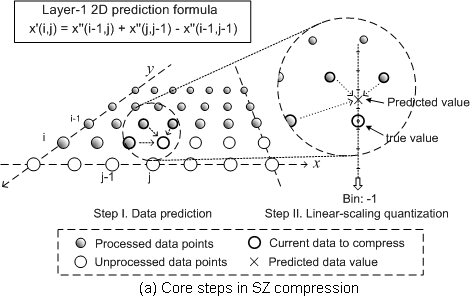
\includegraphics[width=2.8in]{projects/2.3.4-DataViz/2.3.4.14-VeloC-SZ/sz-illu.png}
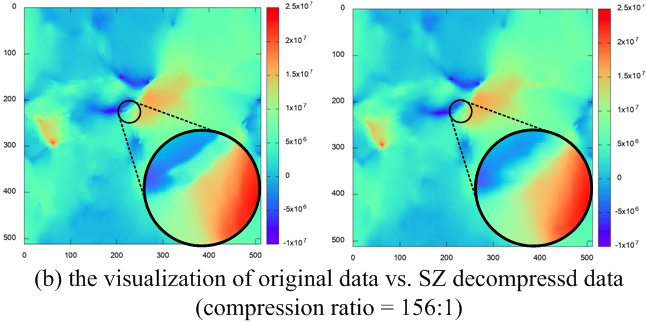
\includegraphics[width=3.2in]{projects/2.3.4-DataViz/2.3.4.14-VeloC-SZ/Visual-quality-NYX-SZ.png}
\vspace{-2mm}
	\caption{\label{fig:sz-principle} SZ principle and  original vs. decompressed NYX VX field}
\end{figure}

We have improved the compression quality for different ECP applications significantly, including ECP HACC, EXAFEL, GAMESS, and others. For instance, SZ leads to higher compression ratio for asbolute error bound on these datasets than the second best lossy compressor, with comparative compression rate. We also implemented effective compression method supporting point-wise relative error bounds for the ECP ExaSky project. Experiments with point-wise relative error bound based compression shows that our solution leads to 31\%-210\% higher compression ratio than other lossy compressors do (best paper at IEEE CLUSTER18). We accelerated the compression rate significantly (by 50\% in most of cases) by a table-lookup method, which was published in IEEE MSST19. 
Moreover, SZ allows users to customize their own prediction method to adapt to the special features of datasets. For instance, the compression ratio has been improved about 2$\sim$3X by leveraging the patterns existing in the GAMESS dataset (overall best paper award at IEEE Cluster 2018).  

All the improvements and functionalities developed in SZ comes from user practical requirements. SZ supports multiple I/O libraries such as HDF5, PnetCDF, and ADIOS; and it also supports both C and Fortran. We also developed various parallel versions such as multi-threaded version and GPU version. SZ also supports random access during the data decompression, allowing users to decompress only interesting regions/parts of the data. We also optimized the I/O performance by exploring the best tradeoff between the compression ratio and compression rate, also taking into account the varied bandwidth with increasing execution scales. This work was published in IEEE Cluster 2019.

\paragraph{Next Steps} Our next efforts are: Improve compression performance by analyzing SZ's performance, refactoring SZ in C++, integrating SZ in more ECP applications, and implementing a portable GPU version for Aurora and Frontier and improving SZ testing environment.

%\textbf{Support advanced error controls allowing the user to specify relative error bounds and to control the error distribution.} We will write a report describing the integration of additional error controls (relative error bound and control of error distribution) in SZ.
